\documentclass[../../main.tex]{subfiles}
\begin{document}

\subsection{Microcontroller} \label{subsec:SystemImplementationMicroController}

\subsubsection*{System overview}
\label{subsec:SystemImplementationOperatingSystem}
It is imperative that the microcontroller is in control of the overall timing of the system. Therefore, the microcontroller is responsible for pulling data from specific slaves on the FPGA. As described in section \ref{sec:Requirements}, it is decided to accommodate a cascaded controller design consisting of two PID-controllers on each motor. This yields a total of four tasks needed to be scheduled regarding the motor control. Furthermore the microcontroller also needs to handle the user interface. The program will be structured as seen on figure \ref{fig:OverviewTaskDiagramSimple}. The task diagram is simplified displaying only one of the cascaded controllers for controlling only one motor, as the second cascaded controller is identical in structure. A more detailed task diagram can be found in the digital appendix section \ref{sec:digital_appendix}. In FreeRTOS tasks have assigned a priority, meaning that high priority tasks are ensured to be scheduled and completed before tasks of lower priority can be scheduled. To achieve a real-time system prioritisation of tasks is vital.

% task will have presedence over lower priority tasks.. 

% Since the PID-controllers need to be processed at a fixed time-interval, as mentioned in section \ref{}, they will have the highest priority after the SPI task.



%This results in four tasks that need to run with predetermined time intervals in real-time. Furthermore a User interface (UI) task for handling user input and a SPI task for sending and receiving data, will need CPU time. By assigning a lower priority to the UI and SPI tasks it is ensured that tasks with higher priority is prioritised when scheduling. This would also keep timing of the time critical controller tasks intact. 

%For the PID-controllers to be able to receive data from the FPGA, SPI is used as mentioned in section \ref{subsec:SystemImplemtationFPGA}. When data is received from the slaves, it is put in buffers accessible only by specific controllers in order for the cascade control to work. To avoid critical section problems with several tasks trying to access the same buffers at the same time, mutex' is implemented. Output from each cascade must then go back to SPI for it to be delivered to the correct slaves. Figure (\ref{fig:OverviewTaskDiagramSimple}) shows a simple overview of the tasks and how they are coupled. A more detailed task diagram can be found in the digital appendix section \ref{sec:digital_appendix}.

% System clock frequency set to 80Mhz
\begin{figure}[H]
    \centering
    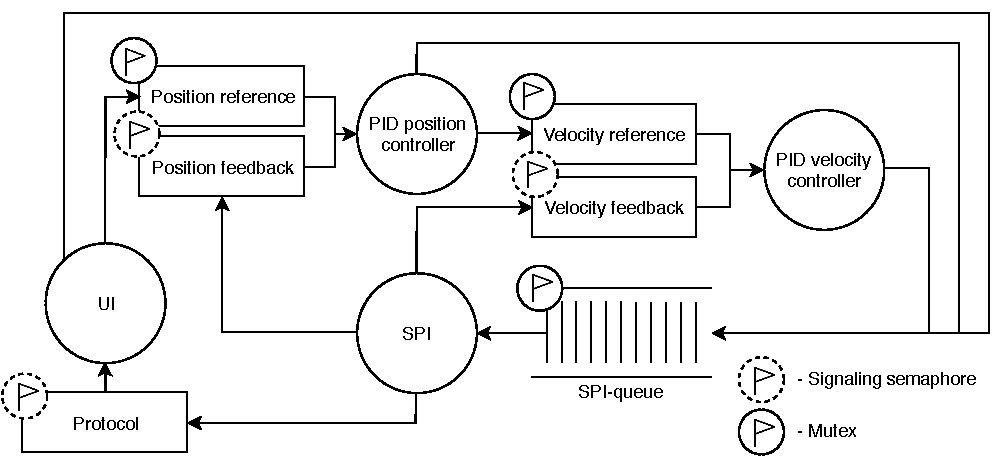
\includegraphics[width=\textwidth]{Sections/System_Implementation/Images/OverviewTaskDiagramSimple.pdf}
    \caption{Simplified task diagram showing the different tasks running on the microcontroller.}
    \label{fig:OverviewTaskDiagramSimple}
\end{figure}






% \subsubsection*{Discrete PID-controller}
% To implement a PID-controller on the microcontroller, it must be discretized. As described in section \ref{sec:Analysis} the Tustin's method is used.
% %Bodeplot til at finde cl båndbredde til at finde minimums samplings frequency
% From equation \ref{eq:eq:discrete_control} it is apparent that the controller is dependant on the sampling time $T$, which on the microcontroller is determined by how often data is requested from the slaves. The minimum sampling time is controlled by how often data is sampled and updated on the FGPA. Velocity data is sampled on each encoder edge, with 1080 encoder ticks every revolution with a duration of \SI{0,88}{\second} \cite{} at maximum velocity, the minimum sampling time is:
% \begin{equation}
%     T_{min} = \frac{0.88\,\mathrm{s}}{1080} = 0.814\,\mathrm{ms}
% \end{equation}
% The maximum sampling time for a smooth response of the discrete controller, need to be 20 to 30 times that of the closed-loop bandwidth(LINK). From figure (ref) $T_{max}$ is found to be:
% \begin{equation}
%     T_{max} = \frac{1}{\omega_b\cdot 30} = \frac{1}{3 \cdot 30} \approx 11.1\,\mathrm{ms}
% \end{equation}
% In a cascade coupling the inner controller has to update faster than the outermost. To comply with this and making sure that $T_{min} > T > T_{max}$, the sampling time for the velocity controller is chosen to be $T_{vel} = 1\,\mathrm{ms}$ and the sampling time for the position controller is $T_{pos} = 5\,\mathrm{ms}$. \\




\subsubsection*{PID-controller Tasks}
% How and which values need to be transported where Reference output controlling PWM
The PID-controller tasks on the microcontroller are responsible for calculating the control signal, which is used to control voltage supplied to the motors. As seen on figure \ref{fig:OverviewTaskDiagramSimple} each controller needs three state buffers, two for input and one for the output. The velocity controller outputs to the SPI-queue. The PID-controller is responsible for requesting data when it is needed. To request feedback data, the controller needs to signal the SPI task via the SPI-queue. When the feedback data is available, the controller task is signaled with a semaphore connected to the feedback state buffer. When the controller is waiting for feedback data to be updated the task enters the blocked state, where it uses no CPU resources. 


% For each controller to be able to function they need three buffers. One buffer holding a reference value and another providing a feedback value. The third buffer is responsible for storing the controller output. In case of a velocity controller the reference buffer contains output from a position controller, while the output buffer is a queue passing on values to SPI. 
% Each buffer has a mutex attached which needs to be waited for or signaled upon using. Figure \ref{fig:OverviewTaskDiagramSimple} constitutes an illustration of the implementation of two PID-controllers in cascade for a single motor. In the actual implementation there are two cascade controllers, one for each motor.

% Following the controller task functionality described on figure  \ref{fig:PIDControllerFlowchart}, feedback to a controller is supplied whenever the controller sends a request to SPI. The request must contain a slave ID indicating which slave to receive data from. The controller task is then put in a blocked state, while waiting for data. Whenever SPI signals that the requested data is put in the feedback buffer associated with the requesting controller, the controller task is put back into running state. 
%As mentioned in section \ref{subsec:SystemImplemtationFPGA}, because of possible variance in velocity feedback due to error in interfacing in the encoder, a second order lowpass Finite Impulse Response (FIR) filter is applied to the error. 

The overall flow of the PID-controller task can be seen on figure \ref{fig:PIDControllerFlowchart}. When the feedback data is received, the error between the reference value and feedback value is calculated. Because the derivative term of the PID-controller amplifies noise, it is beneficial to include a low pass filter in the implementation. The filter can be used specifically on the derivative term, or be applied to the error signal passed to all three terms. Initially the latter approach was implemented, but through tests, it was found that an extra filter specifically on the derivative term was needed as well. Designing these filters has not been highly prioritised and thus not much thought has gone into the filter design. This has been discovered to possibly be a poor prioritisation, and will be discussed in section \ref{sec:Discussion}. The filters are designed using the MATLAB Filter Designer. The filter design seen equation \ref{eq:general_filter},
\begin{equation}\label{eq:general_filter}
    H(z) = \frac{1}{0.0249z^2 + 0.9502z + 0.0249} \qquad ,
\end{equation}
is used for the general error and the design shown in equation \ref{eq:derivative_filter},
\begin{equation}\label{eq:derivative_filter}
    H(z) = \frac{1}{0.0555z^5 + 0.1666z^4 + 0.2777z^3 + 0.2777z^2 + 0.1666z + 0.0555} \qquad ,
\end{equation}
is used for filtering the derivative term.


%It is expected that the signal without any noise would be fairly slow, therefore a low cutoff frequency for the filter is chosen. The sampling frequency for the used filter is \SI{0.5}{\hertz}.
%The transfer function for the filter designed in MATLAB using the filterDesigner:

% The proportional term is then calculated.
%If noise from the encoder is imagined to be a pure sine wave at a single frequency $\omega_a$, then by differentiating the noise described by equation \ref{eq:Sin_noise} it is seen that the amplitude, is multiplied with the frequency $\omega_a$ demonstrating that high frequency noise can ruin performance of the system. 


%Because of this to further dampen the noise, a fifth order lowpass FIR filter is applied to the derivative term, with a cutoff frequency at \SI{0.5}{\hertz}. The transfer function used MATLAB using the filterDesigner is:

%The use of filters when implementing a controller was initially not assumed to be of high importance, when aiming to achieve good system response. Later this has been discovered to be a wrong assumption and that the choices regarding design of the filters have been poor. In section \ref{sec:Discussion} design of filters will be discussed.



% \begin{equation}\label{eq:Sin_noise}
%     \begin{split}
%         y_{noise}(t) &= A\cdot sin(\omega_a t+\phi_a)\\
%         \frac{dy_{noise}(t)}{dt}&=A\cdot\omega_a\cdot sin(\omega_a t+\phi_a+90\degree)
%     \end{split}
% \end{equation}
% where $A$ is the amplitude, $\omega_a$ is the frequency, $\phi_a$ is the phase and $t$ is the time.

To make sure the integral term does not wind up when an error is present for an extended period of time, anti-windup by conditional integration is implemented. As seen on figure \ref{fig:PIDControllerFlowchart} the controller performs a saturation check before updating the output buffer. If the calculated output is in saturation, a flag is raised and the output is set to either the negative or positive saturation value, depending on the sign of the error. On the position controller the saturation limit is equal to the maximum angular velocity, found by test to be approximately \SI{20}{\radian\per\second}, of the pan-tilt system. The saturation limit of the velocity controller is equal to the maximum voltage possible to supply the motors which is either \SI{12}{\volt} or \SI{-12}{\volt}.

\begin{figure}[H]
    \centering
    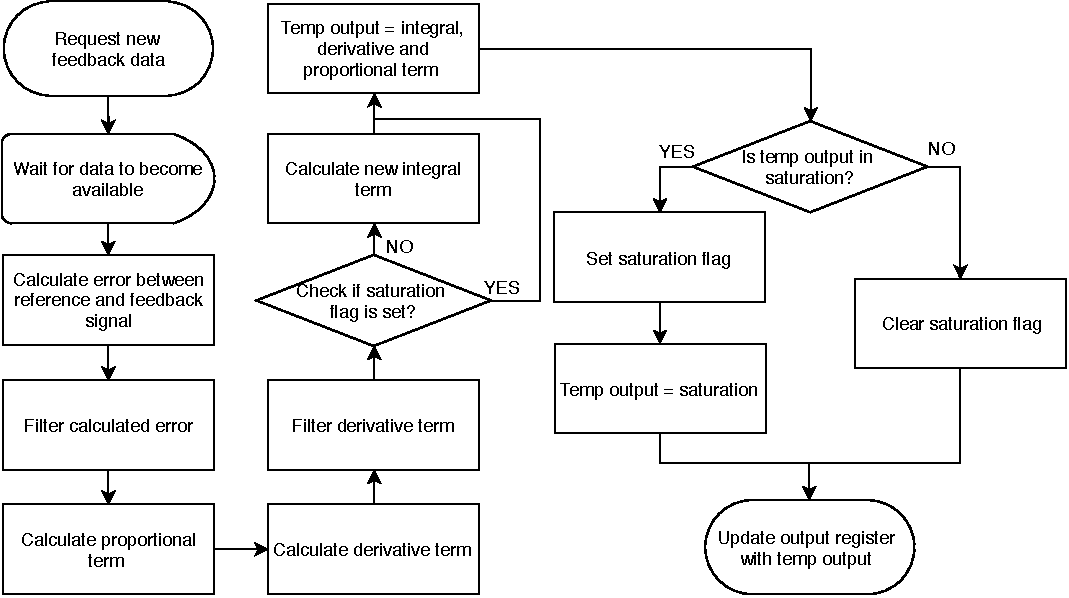
\includegraphics[width=\textwidth]{Sections/System_Implementation/Images/PIDControllerFlowchart.pdf}
    \caption{Flowchart describing the code execution in the PID-controller-task on the microcontroller.}
    \label{fig:PIDControllerFlowchart}
\end{figure}

\subsubsection*{SPI Task}
%Responsibility and purpose of task 
%- PID skal kunne modtage data bestemt efter slave ID. For at det kunne det skal buffers være associeret tilknyttet de buffer.

For the PID-controllers to be able to get their respective feedback data, a SPI task is necessary. To 
he task must handle request from the controllers for getting data from a specific slave.

The microcontroller have build in hardware that enables it to transmit and receive data using SPI. The microcontroller is set up as a master, as described in section \ref{subsec:SystemImplemtationFPGA}. To select a desired slave, the 4-bit address is used. Four general purpose input output pins on the microcontroller are used for selecting a slave, while a hardware controlled pin connected to SPI, is used to enable the slaves. The microcontroller uses a bit rate of \SI{13.3}{\mega bit} when communicating with the slaves on the FPGA. 

% Describe associated buffer/ Hver slave repræsenterer en type info og har derfor en buffer tilknyttet. Beskriv prioritet

As default the SPI task is in the blocked state. Only when a request from one of the controllers enters the SPI-queue, as seen on figure \ref{fig:OverviewTaskDiagramSimple}, the task is given CPU time. Following figure \ref{fig:SPIFlowchart} the request taken from the queue contains a slave ID and data. When the appropriate slave is selected, determined by the slave ID, both data is transmitted and received. If the slave ID has an associated buffer, then the received data is put in that buffer signalling a PID-controller.  

\begin{figure}[H]
    \centering
    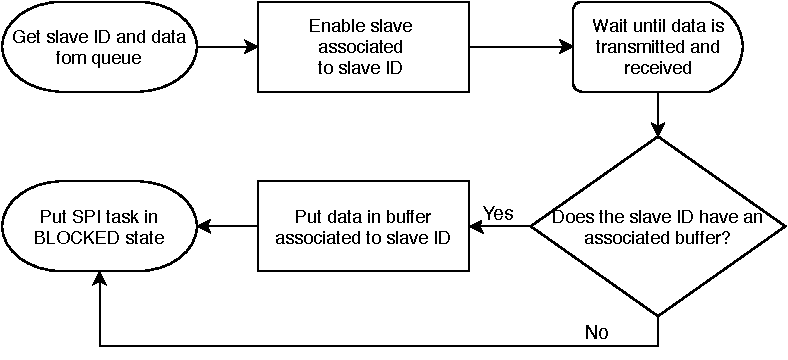
\includegraphics[width=0.8\textwidth]{Sections/System_Implementation/Images/SPIFlowchart.pdf}
    \caption{Flowchart describing the code execution in the SPI task on the microcontroller.}
    \label{fig:SPIFlowchart}
\end{figure}

The SPI task is responsible for providing the PID-controllers with values with units same as the reference value. A conversion has to happen so the units match \[ \left[ \dot{\theta}_m \right] = \SI{}{\radian \per \second }\qquad . \] The motor encoder on the motor has 360 encoder counts per revolution, which means that the relation between the angle of the motor measured in radians and the encoder ticks is, $\pi / 180$. As a result the conversion that is made on the microcontroller is given by equation \ref{eq:velocity_motor}.
\begin{equation}\label{eq:velocity_motor}
    \dot{\theta}_{m} = \frac{\frac{\pi}{180}}{ \dot{\theta}_{\mathrm{FPGA}} }\cdot 10^{5}
\end{equation}


The gearing between the motor and the frame on the robot is 1:3, so the frame experiences one revolution for every three revolutions the motor experiences. The angle of the motor, $ \theta_{m} $, is described by equation \ref{eq:angle_of_motor}, where $FPGA_{pos}$ is the encoder value provided by the FPGA.
\begin{equation}\label{eq:angle_of_motor}
     \theta_{m} = \frac{\pi}{180} \cdot \mathrm{FPGA_{pos}}
\end{equation}


% However a conversion is made in the microcontroller to convert the result to have the units \[ \left[ \dot{\theta}_m \right] = \SI{}{\radian \per \second } \] with respect to the motor. The motor encoder on the motor has 360 encoder ticks per revolution, which means that the relation between the angle of the motor measured in radians and the encoder ticks is, $\pi / 180$. As a result the conversion that is made microcontroller is given by equation \ref{eq:velocity_motor}.
% \begin{equation}\label{eq:velocity_motor}
%     \dot{\theta}_{m} = \frac{\frac{\pi}{180}}{ \dot{\theta}_{\mathrm{FPGA}} }\cdot 10^{5}
% \end{equation}





\subsubsection*{UI Task}
The UI task is responsible for handling user inputs including references for the position controllers. Communication is initiated when the user transmits a command through UART to the microcontroller via the computer. The UI task is given lowest priority, meaning it is only given CPU time whenever no other tasks are scheduled. To facilitate user inputs a protocol has been defined for which the different commands are described in table \ref{tab:UART_UI_PROTOCOL}. With these commands the user is able to reset both motors, home a motor or command a motor to go to a given  reference point. The UI-task consists of two states: "Waiting for command" and "Waiting for queue". The state machine is illustrated in figure
\ref{fig:UITaskStateDiagram}. 

\begin{table}[H]
    \centering
    
    \begin{tabular}{l|c|l|p{0.1\textwidth}|c} %{p{0.12\linewidth}p{0.4\textwidth}p{0.38\textwidth}}
              & Byte & Description & ASCII chars & Value  \\
        \hline
        RESET & 0 & BEGIN RESET COMMAND & 1 & "0" \\
        \hline
        HOME MOTOR  & 0 & HOME MOTOR COMMAND & 1 & "1" \\
                    & 1 & Motor number & 1 & 0-1 \\
        \hline
        GO TO POSITION & 0 & GO TO POSITION COMMAND & 1 & "3" \\
            & 1 & Motor number & 1 & 0-1 \\
            & 2,3,4,5 & Encoder position to go to & 4 & 0-1080 \\
        \hline
        ABORT & 0 & ABORT COMMAND & 1 & "4" \\
        \hline
        MAX PWM TILT & 0 & MAX PWM TILT COMMAND & 1 & "5" \\
       & 1 & Direction of rotation of tilt arm & 1 & 0-1
    \end{tabular}    
    
    \caption{UART Protocol showing the different commands available for the user of the system. "Motor number" chooses either the tilt motor ("0") or the pan motor ("1"). Direction of rotation has similar mechanics where "0" chooses CCW rotation and "1" chooses CW rotation of the tilt arm.}
    \label{tab:UART_UI_PROTOCOL}
\end{table}

\begin{figure}[H]
    \centering
    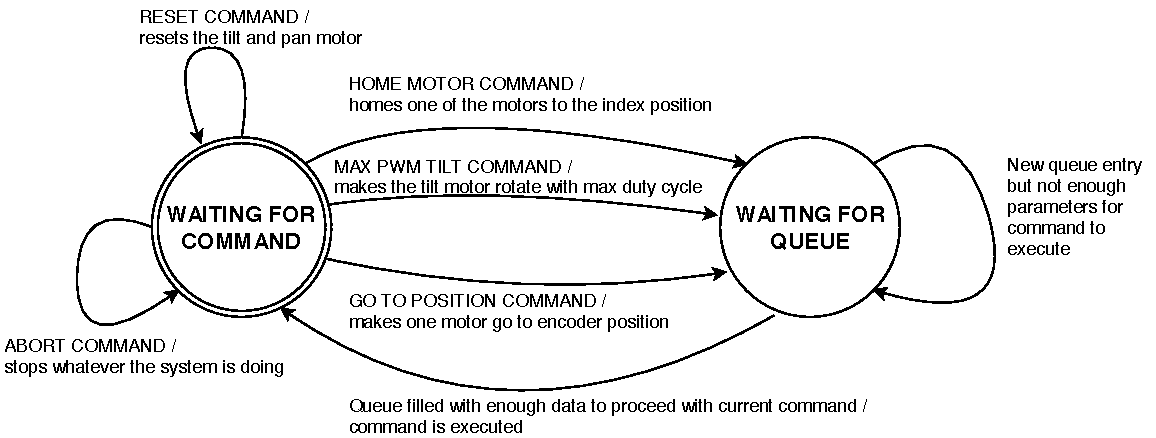
\includegraphics[width=\textwidth]{Sections/System_Implementation/Images/UITaskStateDiagram.pdf}
    \caption{State diagram for the UI task on the microcontroller.}
    \label{fig:UITaskStateDiagram}
\end{figure}




\subsection{Conclusion}
%Which tasks have been implemented, mention slave setup in more detail.

Logic has been implemented on the FPGA to evaluate the position and speed of the motors, to provide a PWM-signal to control the motors and to communicate over SPI with the microcontroller. On the microcontroller FreeRTOS, a real-time operating system, has been implemented for easy separation of algorithms into tasks, that can be scheduled by a scheduling algorithm. Overall the embedded system includes a task to handle the SPI-communication with the FPGA, a task to handle UART-commands sent by the user and tasks to implement the four PID-controllers.   


\end{document}